% mnras_template.tex 
%
% LaTeX template for creating an MNRAS paper
%
% v3.3 released April 2024
% (version numbers match those of mnras.cls)
%
% Copyright (C) Royal Astronomical Society 2015
% Authors:
% Keith T. Smith (Royal Astronomical Society)

% Change log
%
% v3.3 April 2024
%   Updated \pubyear to print the current year automatically
% v3.2 July 2023
%	Updated guidance on use of amssymb package
% v3.0 May 2015
%    Renamed to match the new package name
%    Version number matches mnras.cls
%    A few minor tweaks to wording
% v1.0 September 2013
%    Beta testing only - never publicly released
%    First version: a simple (ish) template for creating an MNRAS paper

%%%%%%%%%%%%%%%%%%%%%%%%%%%%%%%%%%%%%%%%%%%%%%%%%%
% Basic setup. Most papers should leave these options alone.
\documentclass[fleqn,usenatbib]{mnras}

% MNRAS is set in Times font. If you don't have this installed (most LaTeX
% installations will be fine) or prefer the old Computer Modern fonts, comment
% out the following line
\usepackage{newtxtext,newtxmath}
% Depending on your LaTeX fonts installation, you might get better results with one of these:
%\usepackage{mathptmx}
%\usepackage{txfonts}

% Use vector fonts, so it zooms properly in on-screen viewing software
% Don't change these lines unless you know what you are doing
\usepackage[T1]{fontenc}

% Allow "Thomas van Noord" and "Simon de Laguarde" and alike to be sorted by "N" and "L" etc. in the bibliography.
% Write the name in the bibliography as "\VAN{Noord}{Van}{van} Noord, Thomas"
\DeclareRobustCommand{\VAN}[3]{#2}
\let\VANthebibliography\thebibliography
\def\thebibliography{\DeclareRobustCommand{\VAN}[3]{##3}\VANthebibliography}


%%%%% AUTHORS - PLACE YOUR OWN PACKAGES HERE %%%%%

% Only include extra packages if you really need them. Avoid using amssymb if newtxmath is enabled, as these packages can cause conflicts. newtxmatch covers the same math symbols while producing a consistent Times New Roman font. Common packages are:
\usepackage{graphicx}	% Including figure files
\usepackage{amsmath}	% Advanced maths commands

%%%%%%%%%%%%%%%%%%%%%%%%%%%%%%%%%%%%%%%%%%%%%%%%%%

%%%%% AUTHORS - PLACE YOUR OWN COMMANDS HERE %%%%%

% Please keep new commands to a minimum, and use \newcommand not \def to avoid
% overwriting existing commands. Example:
%\newcommand{\pcm}{\,cm$^{-2}$}	% per cm-squared

%%%%%%%%%%%%%%%%%%%%%%%%%%%%%%%%%%%%%%%%%%%%%%%%%%

%%%%%%%%%%%%%%%%%%% TITLE PAGE %%%%%%%%%%%%%%%%%%%

% Title of the paper, and the short title which is used in the headers.
% Keep the title short and informative.
\title[Dark Matter Remnant Shape]{Dark Matter Remnant Shape after M31-Milky Way Merger}

% The list of authors, and the short list which is used in the headers.
% If you need two or more lines of authors, add an extra line using \newauthor
\author[E. H. S. Figureido]{
Ethan H. S. Figureido,$^{1}$\thanks{E-mail: efigureido@gmail.com}}



% These dates will be filled out by the publisher
\date{Submission Date: May 08, 2025}

% Prints the current year, for the copyright statements etc. To achieve a fixed year, replace the expression with a number. 
\pubyear{\the\year{}}

% Don't change these lines
\begin{document}
\label{firstpage}
\pagerange{\pageref{firstpage}--\pageref{lastpage}}
\maketitle

%%abstract
\begin{abstract}
    I present ellipticity measurements of a dark matter halo after a recent major merger. Halo shape can become an indicator of a galaxy's recent merger history, which is a key component of modern theories of galaxy evolution. An N-body simulation of the Milky Way, M31, and M33 merger was used, simulating the moments before and after the major merger, for a total of 12 Gyr of simulated time across 802 data snapshots. I measure the axis ratios of the isocontour ellipses for the projections of the combined halo, determining the shape of the halo and observing how it changes with time. It was found that the halo is triaxial immediately after the merger, smoothing to an oblate shape over time, contrasting with the results of similar studies.
    
\end{abstract}


% Select between one and six entries from the list of approved keywords.
% Don't make up new ones.
\begin{keywords}
Major Merger -- R200 Radius -- Hernquist Profile -- Dark Matter Halo -- Halo Shape -- Oblate/Prolate/Triaxial -- Isodensity Contours -- Galaxy -- Galaxy Evolution 
\end{keywords}

%%%%%%%%%%%%%%%%%%%%%%%%%%%%%%%%%%%%%%%%%%%%%%%%%%

%%%%%%%%%%%%%%%%% BODY OF PAPER %%%%%%%%%%%%%%%%%

\section{Introduction}

The bulk of matter in the universe exists as \textbf{dark matter}: a collisionless particle that doesn’t emit radiation and interacts only gravitationally with other matter. Dark matter is structured as an invisible cosmic web that spans the universe. This web stretches across the universe in filaments and sheets. At the intersection of these structures, we find \textbf{Dark Matter Halos} (DMHs). DMHs are nodes in the dark matter web where regular matter tends to pool, and this makes them sites of galaxy formation and evolution. When gravity pulls nodes together, the galaxies encompassed within them merge as well, altering the structure of the DMH and the galaxies encompassed within.

We use here the \citet{Willman_2012} definition of a \textbf{galaxy}: a gravitationally bound set of stars whose properties cannot be explained by a combination of baryons (non-dark matter matter) and Newton’s laws of gravity. \textbf{Galaxy evolution} pertains to the processes that change the properties and structures of a galaxy overtime. In modern theories of galaxy evolution, galaxy mergers are an important component and occur when two or more galaxies collide. A merger is considered a \textbf{major merger} when the galaxies involved in the collision are of about equal mass. As they are the sites of galaxy evolution, DMH properties are tightly linked to the evolutionary history and properties of galaxies. The structure of DMHs is of particular importance. Understanding how different environments produce different halo structures will provide key insight that we can use to understand a galaxy’s merger history \citep{Drakos_2019}. For example, the shape of a halo is connected to the previous major merger, being stretched along the merger axis \citep{Despali_2016}. Understanding what environments different shapes emerge in will help us understand galaxy merger histories and may make them a powerful indicator of a galaxy's merger history.

Modern theories of galaxy evolution have been crafted through galaxy modeling and observation; observation acting to refine the constraints of simulations. Many simulations have been created using different methods and simulating different environments, and it is easy to find a study whose considered simulation favors any of the possible shapes a DMH can have. DMHs take four main \textbf{halo shapes}: spherical, \textbf{oblate}, \textbf{prolate}, and \textbf{triaxial}. An oblate spheroid is a sphere squashed along an axis such that two of its radii are equal and larger than the radius along the axis of squashing, giving it a grapefruit shape, and a prolate spheroid is a sphere stretched along an axis such that two radii are equal but smaller than the radius along the axis of stretching, giving it an American football shape. A triaxial shape is a sphere stretching in two directions such that the radius along each axis is a different length. Using galaxy modeling, we have learned much about these shapes and the environments that favor them. DMHs grow through the accretion of surrounding matter and mergers.  In isolation, this growth is anisotropic, favoring triaxial and prolate DMH shapes over spherical or oblate. If we were to consider baryonic processes like black hole feedback, radiative processes, and star formation, we find a smoother, oblate shape. Fig.~\ref{fig:MHD vs DMO} (Fig.3 from \citet{Prada_2019}) illustrates the effects of baryonic processes on halo shape by comparing the axes ratios of halos from magneto-hydrodynamic simulations, which include baryonic effects, and dark matter only simulations which don't. These simulations provide insight into how halos are shaped by the baryonic matter that they encompass.

Much of the uncertainty in this topic stems from the variety of methods and environments used in galaxy simulations, and inadequate resolution. Furthermore, the exact effects of different baryonic processes on DMHs are yet to be adequately determined. The large variety of environments, assumptions, and uncertainties of different simulations has produced evidence favoring each of the four possible halo shapes, as discussed in \citet{Chua_2019} and \citet{Prada_2019}. Many of the open questions surround the reliability of observations and assumptions used to constrain simulations.

\begin{figure}
	\includegraphics[width=\columnwidth]{fig 3 prada+2019.jpg}
    \caption{Figure 3 from \citet{Prada_2019}. Plotting the axes ratios for 30 simulated DMHs for dark matter only (DMO, left) and magneto-hydrodynamic (MHD, right) simulations. Triangles indicate data for the inner regions (R200/16 (~14kpc)) of the halos. They visualize three main population trends: DMO simulations are rounder in the outer regions than the inner, MHD simulations are rounder in the inner regions than the outer, and MHD halos are rounder than DMO halos, indicating the influence of baryonic matter on the DMH it is encompassed in}
    \label{fig:MHD vs DMO}
\end{figure}


\section{This Project}

In this paper, I will study the shape of the merged DMH remnant after the major merger between the Milky Way (MW) and M31, and how the shape evolves overtime.  

By analyzing the DMH shape, I aim to replicate the findings of other studies like \citet{Drakos_2019}, who found the halo shape to stretch along the direction of the merger, and \citet{Prada_2019} whose results are displayed in Fig.~\ref{fig:MHD vs DMO}.

DMH shapes are linked to the evolutionary history of galaxies. Studying them can reveal trends that we can apply to other galaxies, unveiling their merger histories.



\section{Methods}

This study will be conducted using data from the M31-M33-MW merger simulation found in the \citet{van_der_Marel_2012} study. It is an N-body simulation: a dynamical system of particles under the influence of physical forces, in this case gravity. There are three types of particles considered in this simulation: halo, disk, and bulge particles. The disk and bulge particles represent the baryonic matter components of the star, and the halo particles are the dark matter that surrounds them. Particle position, velocity, and mass data are recorded in a series of 800 snapshots which span approximately 11.5 Gyr, capturing the moments before, during, and after the merger.

Using the high resolution simulation data, I will extract the position data of the halo particles for both M31 and the MW after their merger is completed.  The \textbf{R200 radius} will be used to determine the edge of the halo. By fitting a computed mass profile to a Hernquist profile, we can determine the radius at which the density of the DMH is equal to 200 times the critical density of the universe. The critical density of the universe is defined as follows

\begin{equation} \label{critical density}
    \rho_{crit}=\frac{3H_o^2}{8G\pi}
\end{equation}

Where \begin{math}H_{o}\end{math} is the Hubble parameter, and \begin{math}G\end{math} is the gravitational constant. So we find,

\begin{equation} \label{R200 density}
    \rho(r=R_{200})=200\rho_{crit}=26550 M_\odot /kpc^3
\end{equation}

Taking \begin{math}H_o=68.9\text{ km/s/Mpc}\end{math} to be our Hubble parameter. Using (\ref{R200 density}) with (\ref{hernquist}) we find the halo edge at \begin{math}r=149\text{ kpc}\end{math}.

To determine the ellipticity of each axis, and thus the shape of the DMH, I will use the position data of the simulated halo particles and plot projections against the xy, xz, and yz-planes, fitting an ellipse to an isodensity contour at the edge of the halo using the photutils python package. Fig.~\ref{fig:xy-plane projection} is an example of an xy-plane projection of the merged DMH. This will be done for each snapshot after the merger has been completed. The ellipticity values can be plotted against time, which will allow me to analyze how the shape evolves overtime.


\begin{figure}
	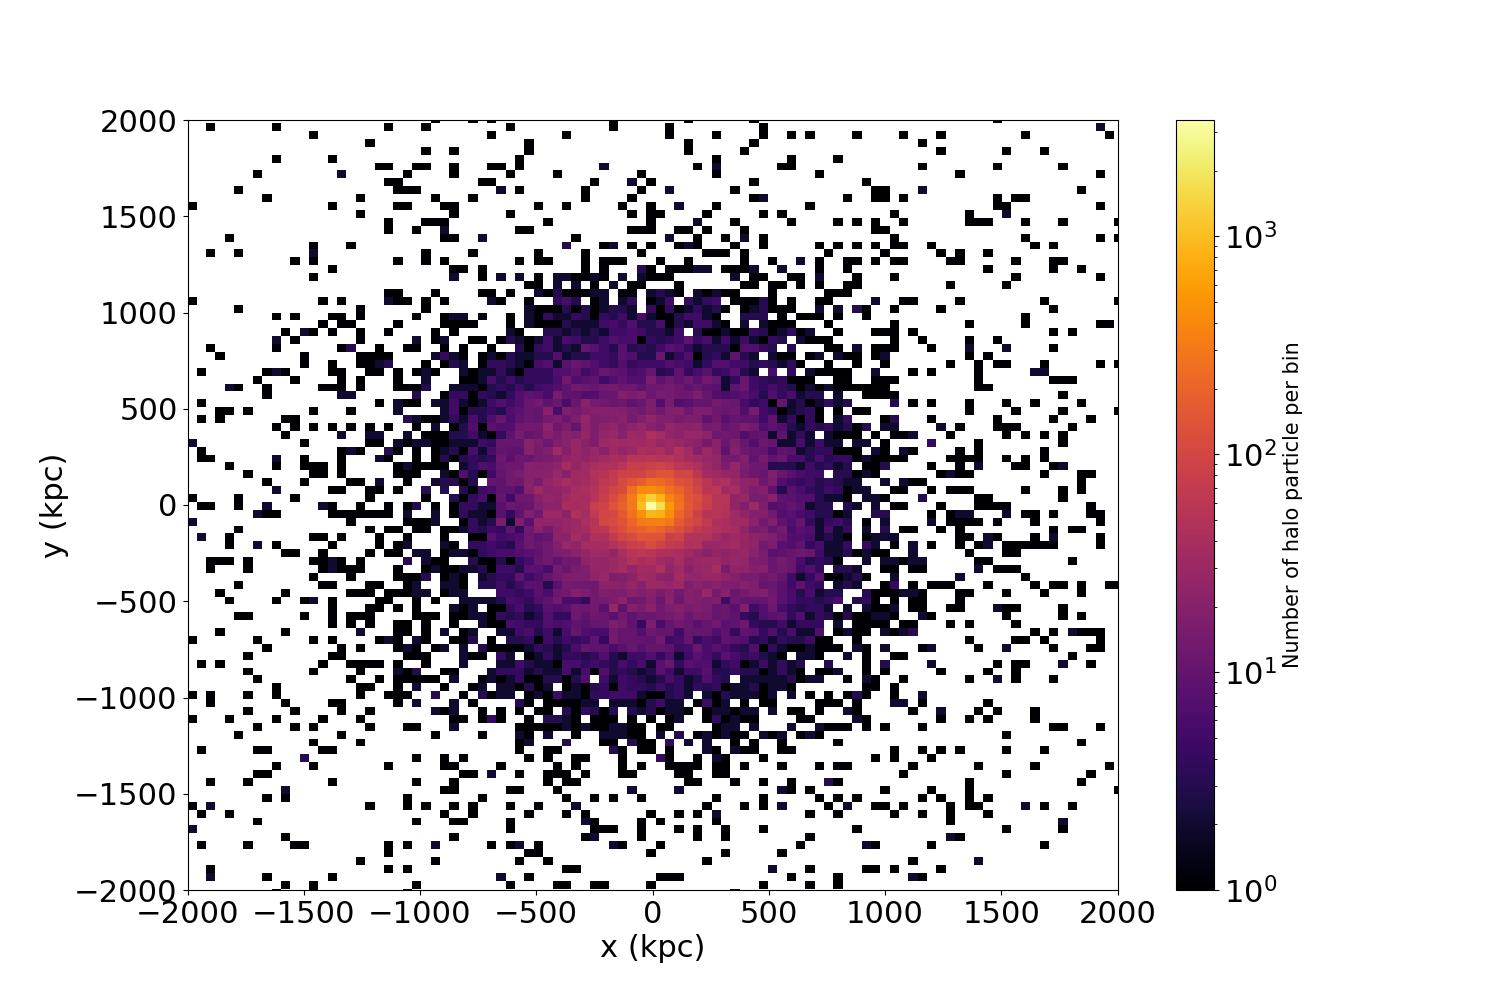
\includegraphics[width=\columnwidth]{xy-projection of halo number density.jpg}
    \caption{Projection of the xy-plane of the merged DMH of the MW and M31 as a 2D number density histogram. It is plotted such that the center of mass is at the origin and the angular momentum vector is aligned in the z-direction. The data is from 8.5 Gyr after the beginning of the simulation and 2.5 Gyr after the merger has completed, corresponding to snapshot 600.}                     
    \label{fig:xy-plane projection}
\end{figure}

There are few calculations that my code will need to be computed to retrieve the necessary data. A density profile must be fitted for the combined DMH remnant, so that the edge of the halo can be determined. Using the \textbf{Hernquist Profile} from \citet{Hernquist_1990}, we will determine a density profile, fitting an isodensity contour to determine the halo edge. The Hernquist Profile is defined as equation (\ref{hernquist}), where \begin{math}M_{halo}\end{math} is the total mass of the DMH, \begin{math}h_a\end{math} is the scale radius of the Hernquist profile, and \begin{math}r\end{math} is the distance from the galactic center. Minimal calculation is needed from here. The virial radius will be found using the Hernquist profile.

\begin{equation} \label{hernquist}
    \rho(r)=\frac{M_{halo}}{2\pi} \frac{h_a}{r(r+h_a)^3}
\end{equation}


The data will be plotted in many different forms to visualize the dark matter distribution. Projections of the xy, xz, and yz-planes of the DMH will be plotted with an ellipse fit to the isodensity contour that agrees with the virial radius, to visualize the ellipticity of the DMH. The axis ratios will be used to determine its shape. Finding the axis ratios for the DMH for each snapshot after the merger has completed will allow for an analysis of the evolution of the shape. By graphing how the axis ratio changes overtime, we can show how its shape evolves immediately after the merger.

From \citet{Despali_2016} a shape elongated along the merger axis is expected. Radiative processes, star formation, and AGN feedback are absent in this simulation. These processes generally smooth the halo to create a more oblate shape, so the simulation is expected to favor a non-oblate shape. Further, because these halos are so large, we expect the growth of the halo to begin with an initially triaxial shape. Combining the above, a triaxial halo with its longest axis in the direction of the merger axis is expected as the merged halo shape.



\section{Results}

By fitting the Hernquist profile of the DMH to its computed mass profile, I found a value of 110 kpc for the scale height of the halo. Using this fitted Hernquist Profile, the R200 radius of the halo was identified at 149 kpc. Isodensity contours were fitted for this radius, defining the edge of the halo in the 3 coordinate planes, as seen in Fig.~\ref{fig:contour fitting}. In this figure, the black ellipse represents the best fit ellipse for a semi-major axis equal to the R200 radius in the xy-projection. The average ellipticity values in each projection over the course of the simulation are: \begin{math} <\epsilon_{xy}>=0.09\end{math}, \begin{math}<\epsilon_{xz}>=0.20\end{math}, and \begin{math}<\epsilon_{yz}>=0.19\end{math}. These data imply an oblate shape on average after the merger.

Fig.~\ref{fig:ellipticity} shows results for how ellipticity and axis ratios change overtime. We see high ellipticities and a sharp decreasing trend early after the merger. The plot shows the DMH takes a triaxial shape that slowly decreases in size until snapshot 550 when the xz and yz ellipticities begin to increase, and the xy bounces around the lower values. We see in this data a similar trend between the xy and yz ellipticities in the early snapshots, before the yz breaks away from the xy and follows the xz-projection trend. Its at this point that the halo shape smooths from triaxial to oblate, as the xz and yz ellipticities converge.


\begin{figure}
	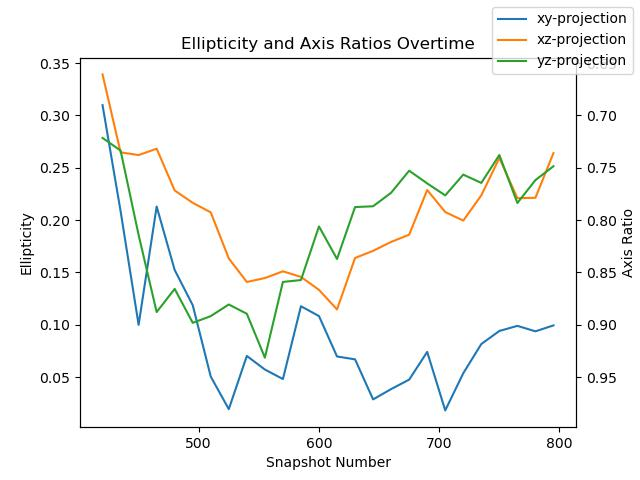
\includegraphics[width=\columnwidth]{Ellipticity and Axis Ratios.jpg}
    \caption{A plot of the ellipticity and axis ratios of the best fit isodensity contours for each projection of the DMH overtime. The left axis is the ellipticity, and the right is the axis ratio. The yellow line is the ellipse in the xz-projection, the green is the yz-projection, and the blue is the xy-projection. Time is plotted on the x-axis as snapshot number from snapshot 420 (6 Gyr) to snapshot 795 (11.35 Gyr). This graph shows that the DMH shape is generally triaxial through time after the merger. However, the axes of stretching for this shape shift around snapshot 600 (8.5 Gyr) converging to an oblate shape. Highest ellipticity is found in the earliest snapshots, as matter was still settling after the merger.}
    \label{fig:ellipticity}
\end{figure}


\begin{figure}
	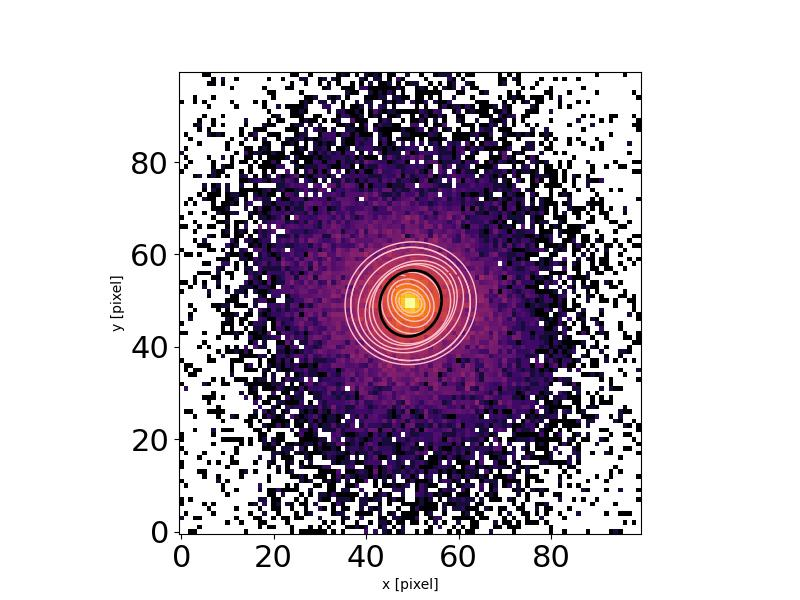
\includegraphics[width=\columnwidth]{halo contour fitting.jpg}
    \caption{A plot of isodensity contours for the xy-projection of the halo at snapshot 600 (8.5 Gyr) on a scale 10 [kpc/pixel]. The pink ellipses represent lines of constant density, for different semi-major axes between 50 and 300 kpc. The black ellipse represents the best fit ellipse with semi-major axis at the edge of the halo as defined by the R200 radius of 149 kpc. For snapshot 600 we have the following ellipticity values: \begin{math}\epsilon_{xy}=0.11\end{math}, \begin{math}\epsilon_{xz}=0.13\end{math}, and \begin{math}\epsilon_{yz}=0.19\end{math}, which gives the halo a triaxial shape.}            
    \label{fig:contour fitting}
\end{figure}


\section{Discussion}

The DMH shape is triaxial immediately after the conclusion of the merger. It remains in triaxial form for an extended period, slowly decreasing in size. At snapshot 550, this triaxial shape begins to smooth out, becoming almost perfectly oblate until the end of the simulation. This disagrees with hypothesis, which predicts an initially triaxial shape that smooths to a prolate one, stretching in the direction of the merger.

These results contradict what is described in \citet{Despali_2016} and the trends found in \citet{Prada_2019}. \citet{Despali_2016} describes a halo shape stretched in the direction of the merger, but we our results show an oblate shape, not stretched in one direction, but squashed in one direction. The data also contradicts what is found in \citet{Prada_2019}. A simulation lacking MHD processes like this one should favor prolate orientations (Fig.~\ref{fig:MHD vs DMO}). It is possible to attain an oblate halo under these conditions, however, and the variable results may be due to the high masses of the Mw and M31. When these two spiral galaxies merge, they become a high-mass elliptical galaxy, and this oblate sphere may match the distribution of baryonic matter better than a prolate shape.

A large source of error in this analysis is due to the resolution of the simulation data, as the low-resolution data was used over the high-resolution. Baryon distribution has an effect on the shape of the halo, and matter densities change significantly between the high and low resolutions. Further, ellipticity data was computed for every 15 snapshots, computing for shorter time periods could smooth trends that appear choppy in the data. Another point to consider is the presence of M33 in the simulation. M33 particle data was not included in the analysis of the MW-M31 halo, but its gravitational effects on the MW and M31 particles are still present. This may have created a perturbation large enough to bias the results, and this was not accounted for in the analysis.


\section{Conclusion}

Presented in this paper are ellipticity values for the shape of the combined DMH of the MW and M31. The simulation from \citet{van_der_Marel_2012} was used in this study: an N-body simulation of the future M31-M33-MW merger. Halo shapes can provide insight into the recent merger history of a galaxy. I seek to understanding how this environment favors its shape, and how the shape changes through time, in order to unlock the history of observed galaxies.

Most interestingly, the results indicate that the halo shape evolves from the triaxial shape it takes immediately after the merger, into an almost perfectly oblate shape as the simulation approaches its final runtime. The final oblate shape contradicts data from other studies, and disagrees with my hypothesis. If we considered the effect of M33 we would expect stretching, but we find a flattening of the shape instead.

It can be seen immediately that this experiment can be improved by using the high resolution data. The issue lies with the code written for this study. The low and high resolution data is formatted identically, so low resolution was used throughout testing to save time. However, when switching to the high resolution,  the code failed, solving this issue would do much for the study. Further, considering the gravitational effect of M33 on the combined halo in the analysis would reduce uncertainty in the data, and it would be interesting to consider an environment that included a satellite galaxy.



\section*{Acknowledgements}
I thank Dr. Gurtina Besla and Himansh Rathore for their help in the writing of code and reviewing of this study. This work was performed using simulation data from the \citet{van_der_Marel_2012} study, the authors of which I thank.

This work made use of the following software packages: \texttt{astropy} \citep{astropy:2013, astropy:2018, astropy:2022}, \texttt{Jupyter} \citep{2007CSE.....9c..21P, kluyver2016jupyter}, \texttt{matplotlib} \citep{Hunter:2007}, \texttt{numpy} \citep{numpy}, \texttt{python} \citep{python}, \texttt{scipy} \citep{2020SciPy-NMeth, scipy_14880408}, and \texttt{scikit-image} \citep{scikit-image}.

This research made use of Photutils, an Astropy package for detection and photometry of astronomical sources \citep{Photutils_14889440}.

Software citation information aggregated using \texttt{\href{https://www.tomwagg.com/software-citation-station/}{The Software Citation Station}} \citep{software-citation-station-paper, software-citation-station-zenodo}.

We respectfully acknowledge the University of Arizona is on the land and territories of Indigenous peoples. Today, Arizona is home to 22 federally recognized tribes, with Tucson being home to the O’odham and the Yaqui. The University strives to build sustainable relationships with sovereign Native Nations and Indigenous communities through education offerings, partnerships, and community service.

%%%%%%%%%%%%%%%%%%%% REFERENCES %%%%%%%%%%%%%%%%%%

% The best way to enter references is to use BibTeX:

\bibliographystyle{mnras}
\bibliography{example} % if your bibtex file is called example.bib


% Alternatively you could enter them by hand, like this:
% This method is tedious and prone to error if you have lots of references
%\begin{thebibliography}{99}
%\bibitem[\protect\citeauthoryear{Author}{2012}]{Author2012}
%Author A.~N., 2013, Journal of Improbable Astronomy, 1, 1
%\bibitem[\protect\citeauthoryear{Others}{2013}]{Others2013}
%Others S., 2012, Journal of Interesting Stuff, 17, 198
%\end{thebibliography}

%%%%%%%%%%%%%%%%%%%%%%%%%%%%%%%%%%%%%%%%%%%%%%%%%%

%%%%%%%%%%%%%%%%% APPENDICES %%%%%%%%%%%%%%%%%%%%%



% Don't change these lines
\bsp	% typesetting comment
\label{lastpage}
\end{document}

% End of mnras_template.tex
